\chapter{FiC-SW}
\section{FiC(Flow-in-Cloud)システム}
FiC(Flow-in-Cloud)システムは、NEDO人工知能プロジェクトにおいて、FPGAノード、GPUノード、メモリノードなどの異種ノードを多数組み合わせた大規模計算システムである。
図\ref{fig_fic1}はFPGA搭載スイッチノード(FiC-SW)を中心としたFiCシステムの構成例を示す。
このシステムはデータフローによって各ノードが動作し、目的の処理が進められるようになっている。
図\ref{fig_fic2}はFPGA、GPU、メモリを組み合わせ機械学習処理を行うシステムの構成例である。

さらに、FiCシステムでは、各ノード間の接続は低コストなサーキットスイッチングで行う。
これは、通信の帯域を保証することで、このシステム上で動作する専用のシステムソフトウェアのオーバーヘッドを可能な限り減少させ、アプリケーションを高速化させる狙いがある。

\begin{figure}[ht]  
 \begin{center}   
	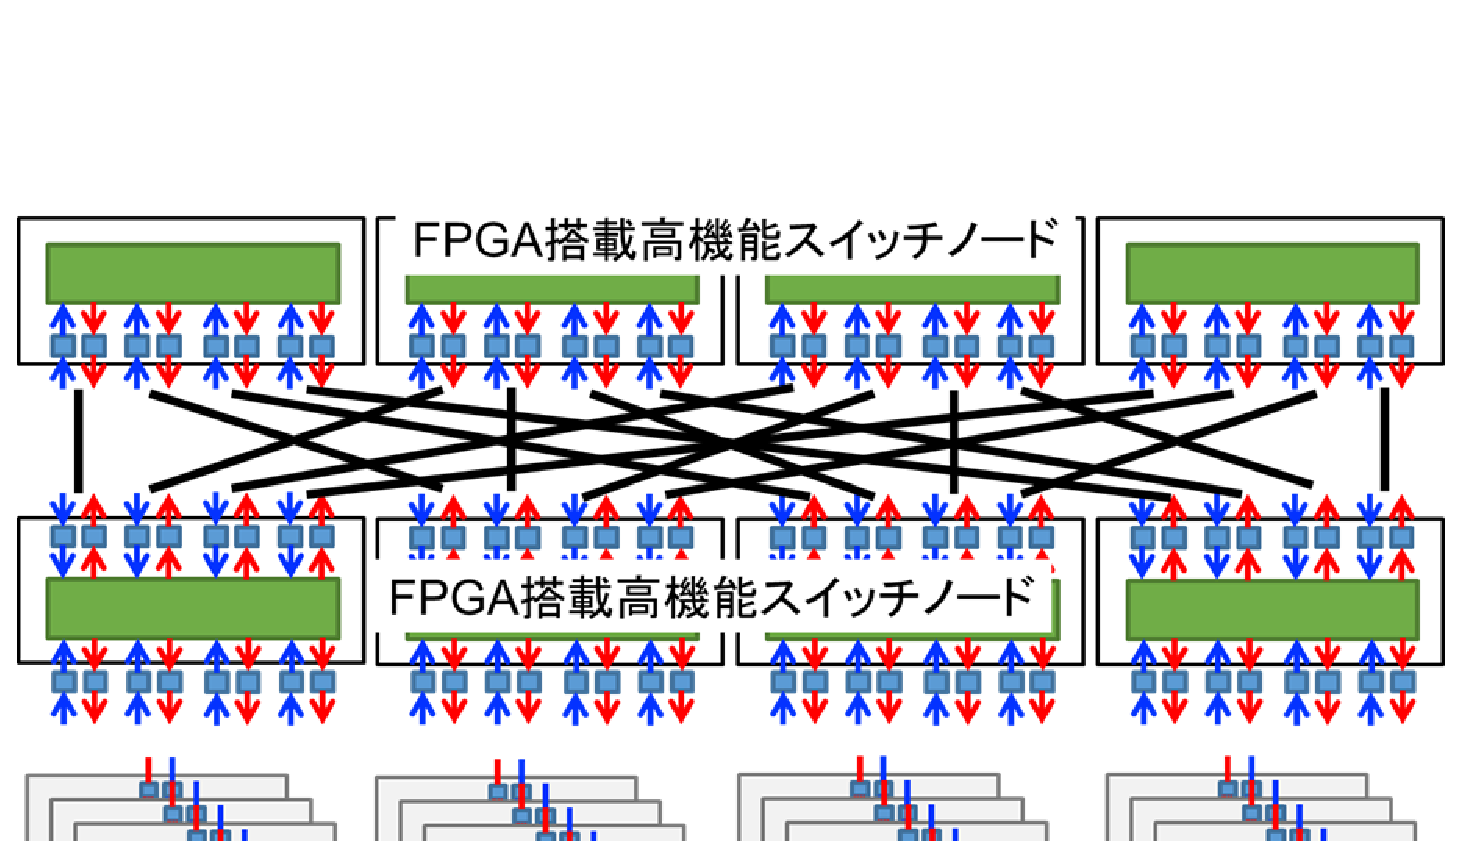
\includegraphics[width=1.0\columnwidth]{fig/FiC.eps}
  \caption{FiCの構成例}
%  \ecaption{Static analysis result of an example pattern}
  \label{fig_fic1}  
 \end{center}  
\end{figure}

\begin{figure}[ht]  
 \begin{center}   
	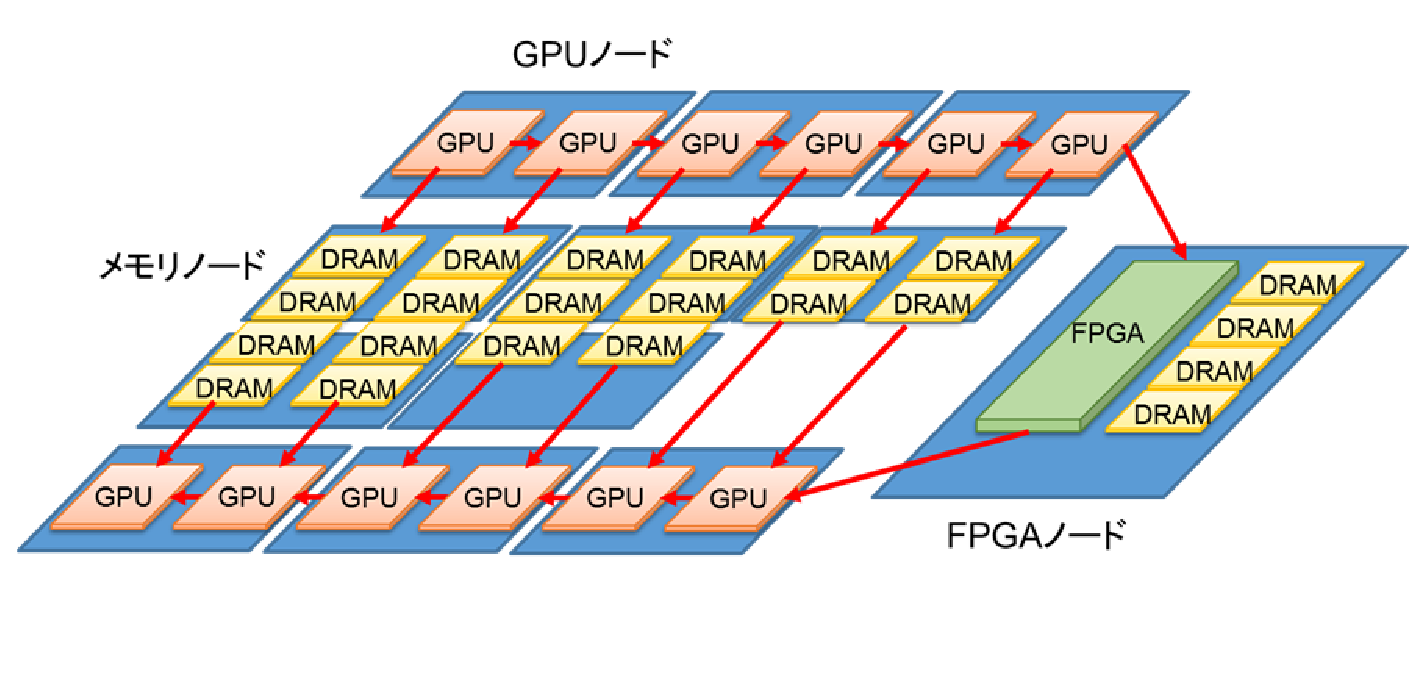
\includegraphics[width=1.0\columnwidth]{fig/example.eps}
  \caption{FiCによる学習システム構成例}
%  \ecaption{Static analysis result of an example pattern}
  \label{fig_fic2}  
 \end{center}  
\end{figure}

\section{FiC-SW1}
FiC-SW1は、初期のソフトウェア開発用のテストベッドのために使う、高速リンクを多数接続したFPGAボードである。
このFiC-SW1ボードはシステムソフトウェア開発用テストベッドとしての役割だけだでなく、
将来のFiCシステムのスイッチングハブとしての役割、GPU開発が完了するまでの演算コアとしての役割もある。


図\ref{fig_sw1}に現在開発中のFiC-SW1ボードの構成を示す。
FPGAにはXilinx社のKintex Ultrascale KU095を用いる。
ストレージとしてはDDR-4 SDRAM16GBを4組持つ。
ボード間接続のためには8Gbpsの高速光シリアルリンクを8組装備する。
リンクは全二重のため、合計の転送容量は16Gbpsとなる。

また、制御用に制御用に RaspberryPi 3 ボードをドーターボードの形で接続する。FPGAの再構成などはこのRasPi3からEthernet経由で行う。

\begin{figure}[ht]  
 \begin{center}   
	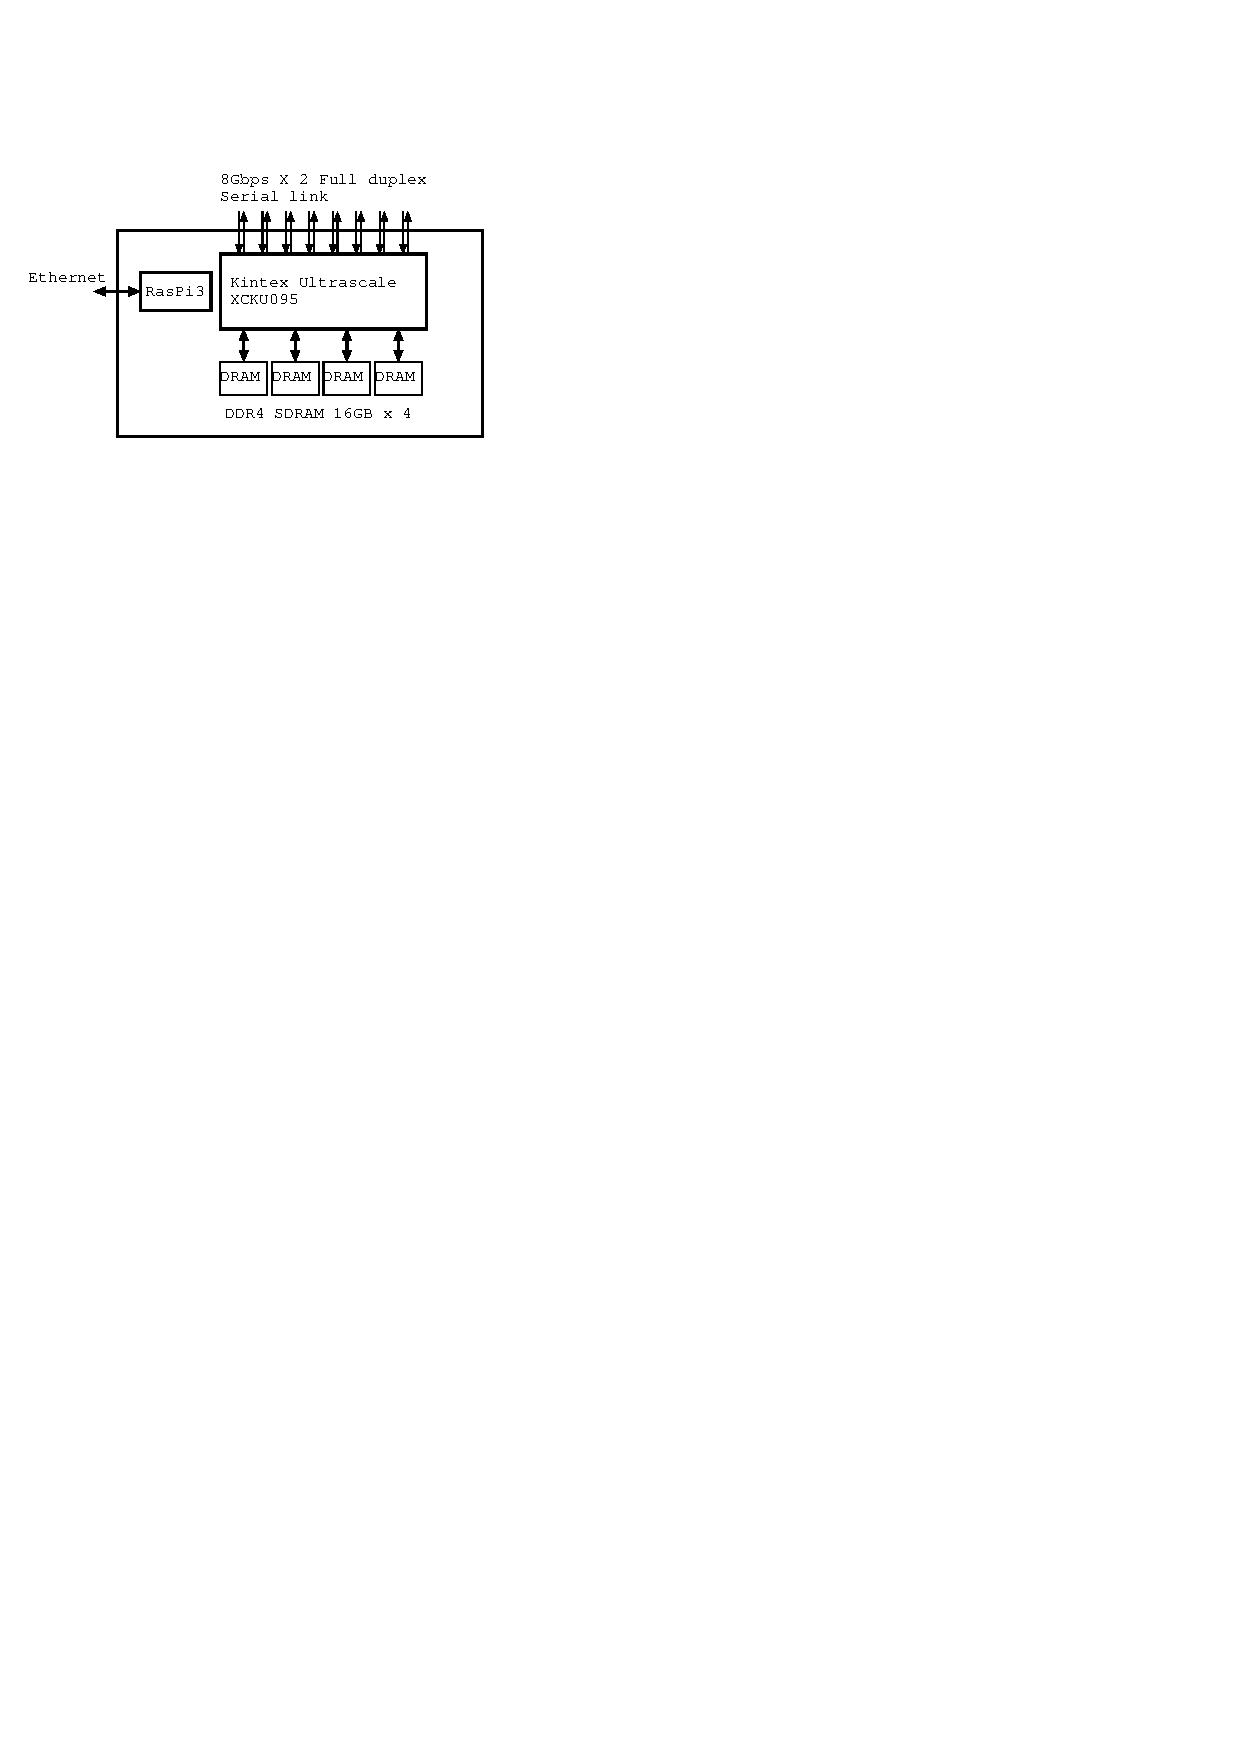
\includegraphics[width=1.0\columnwidth,bb=0 0 720 540]{img/ficsw1.png}
  \caption{FiC-SW1ボードの構成}
%  \ecaption{Static analysis result of an example pattern}
  \label{fig_sw1}  
 \end{center}  
\end{figure}

\section{FiC-SW1のサーキットスイッチング}
FiCシステムでのスイッチノードの役割も持つFiC-SW1ボードのサーキットスイッチングによる通信についてを解説する。

サーキットスイッチングとは、通信の前に事前に通信路を設定し、一定の帯域を占有してから送受信を行う通信の方式である。
FiCシステムが扱う機械学習アルゴリズムの多くは、1対1、1対全、全対全など、特定の通信路をあからじめ予測することが可能である。
そのため、通信帯域と通信遅延を保証することができるサーキットスイッチングがFiC-SW1には採用された。

図\ref{fig_switch}はFiC-SW1のスイッチの概要図である。このスイッチが1サイクルあたりに受信する転送データを格納する容量を持つバッファとして「スロット」を定義する。
そして、図\ref{fig_switch}にように入出力スロット間の接続によって経路を構成する。経路は1対1だけでなく、1対多が可能で、効率的にマルチキャストできる。
各ポートでは、1サイクルごとに順番にスロットを巡回して送受信を行うことで時分割多重(TDM : Time Division Multiplexing)を実現する。
各スロットの読み書きは同期を取らず、RAWハザード(データ書き込み前にデータ読み込みをしてしまうエラー)と、WARハザード(データ読み込み前にデータ書き換えをしてしまうエラー)のみを保証するだけで十分である。

スイッチのポートには隣接するスイッチに繋がるものと、FPGAなどの計算ノードに繋がるものが存在する。

このスイッチでは、スロットの書き込み位置によって経路が一意に決定されるよう事前に経路を設定しなければならない。
入出力スロット間の接続や再接続には、FiC-SW1内部向けに用意されたスロットへ特定の値を書き込むことで行われる。
図\ref{fig_multicast}は、1対2通信を利用してこのスロットに値を書き込み、マルチキャストへと接続を再構成している例である。
このように、定期的に入出力スロット間の接続は更新することが可能となっている。
ただし、内部向けのこのスロットは、FiC-SW1上で演算を行う際の入出力が本来の目的である。

このように、現状のFiC-SW1ボードでは光リンクと電気スイッチによってサーキットスイッチングを行う。
しかし、FiCシステムでは将来的に、光ネットワークを採用したより高速な相互通信を行う計画がある。
そのため、この電気スイッチは、光スイッチに置き変えられることを想定して設計された。
この場合、時分割多重は波長多重に置き変えられ、1スロットは1チャンネルに相当することになる。

\begin{figure}[ht]  
 \begin{center}   
	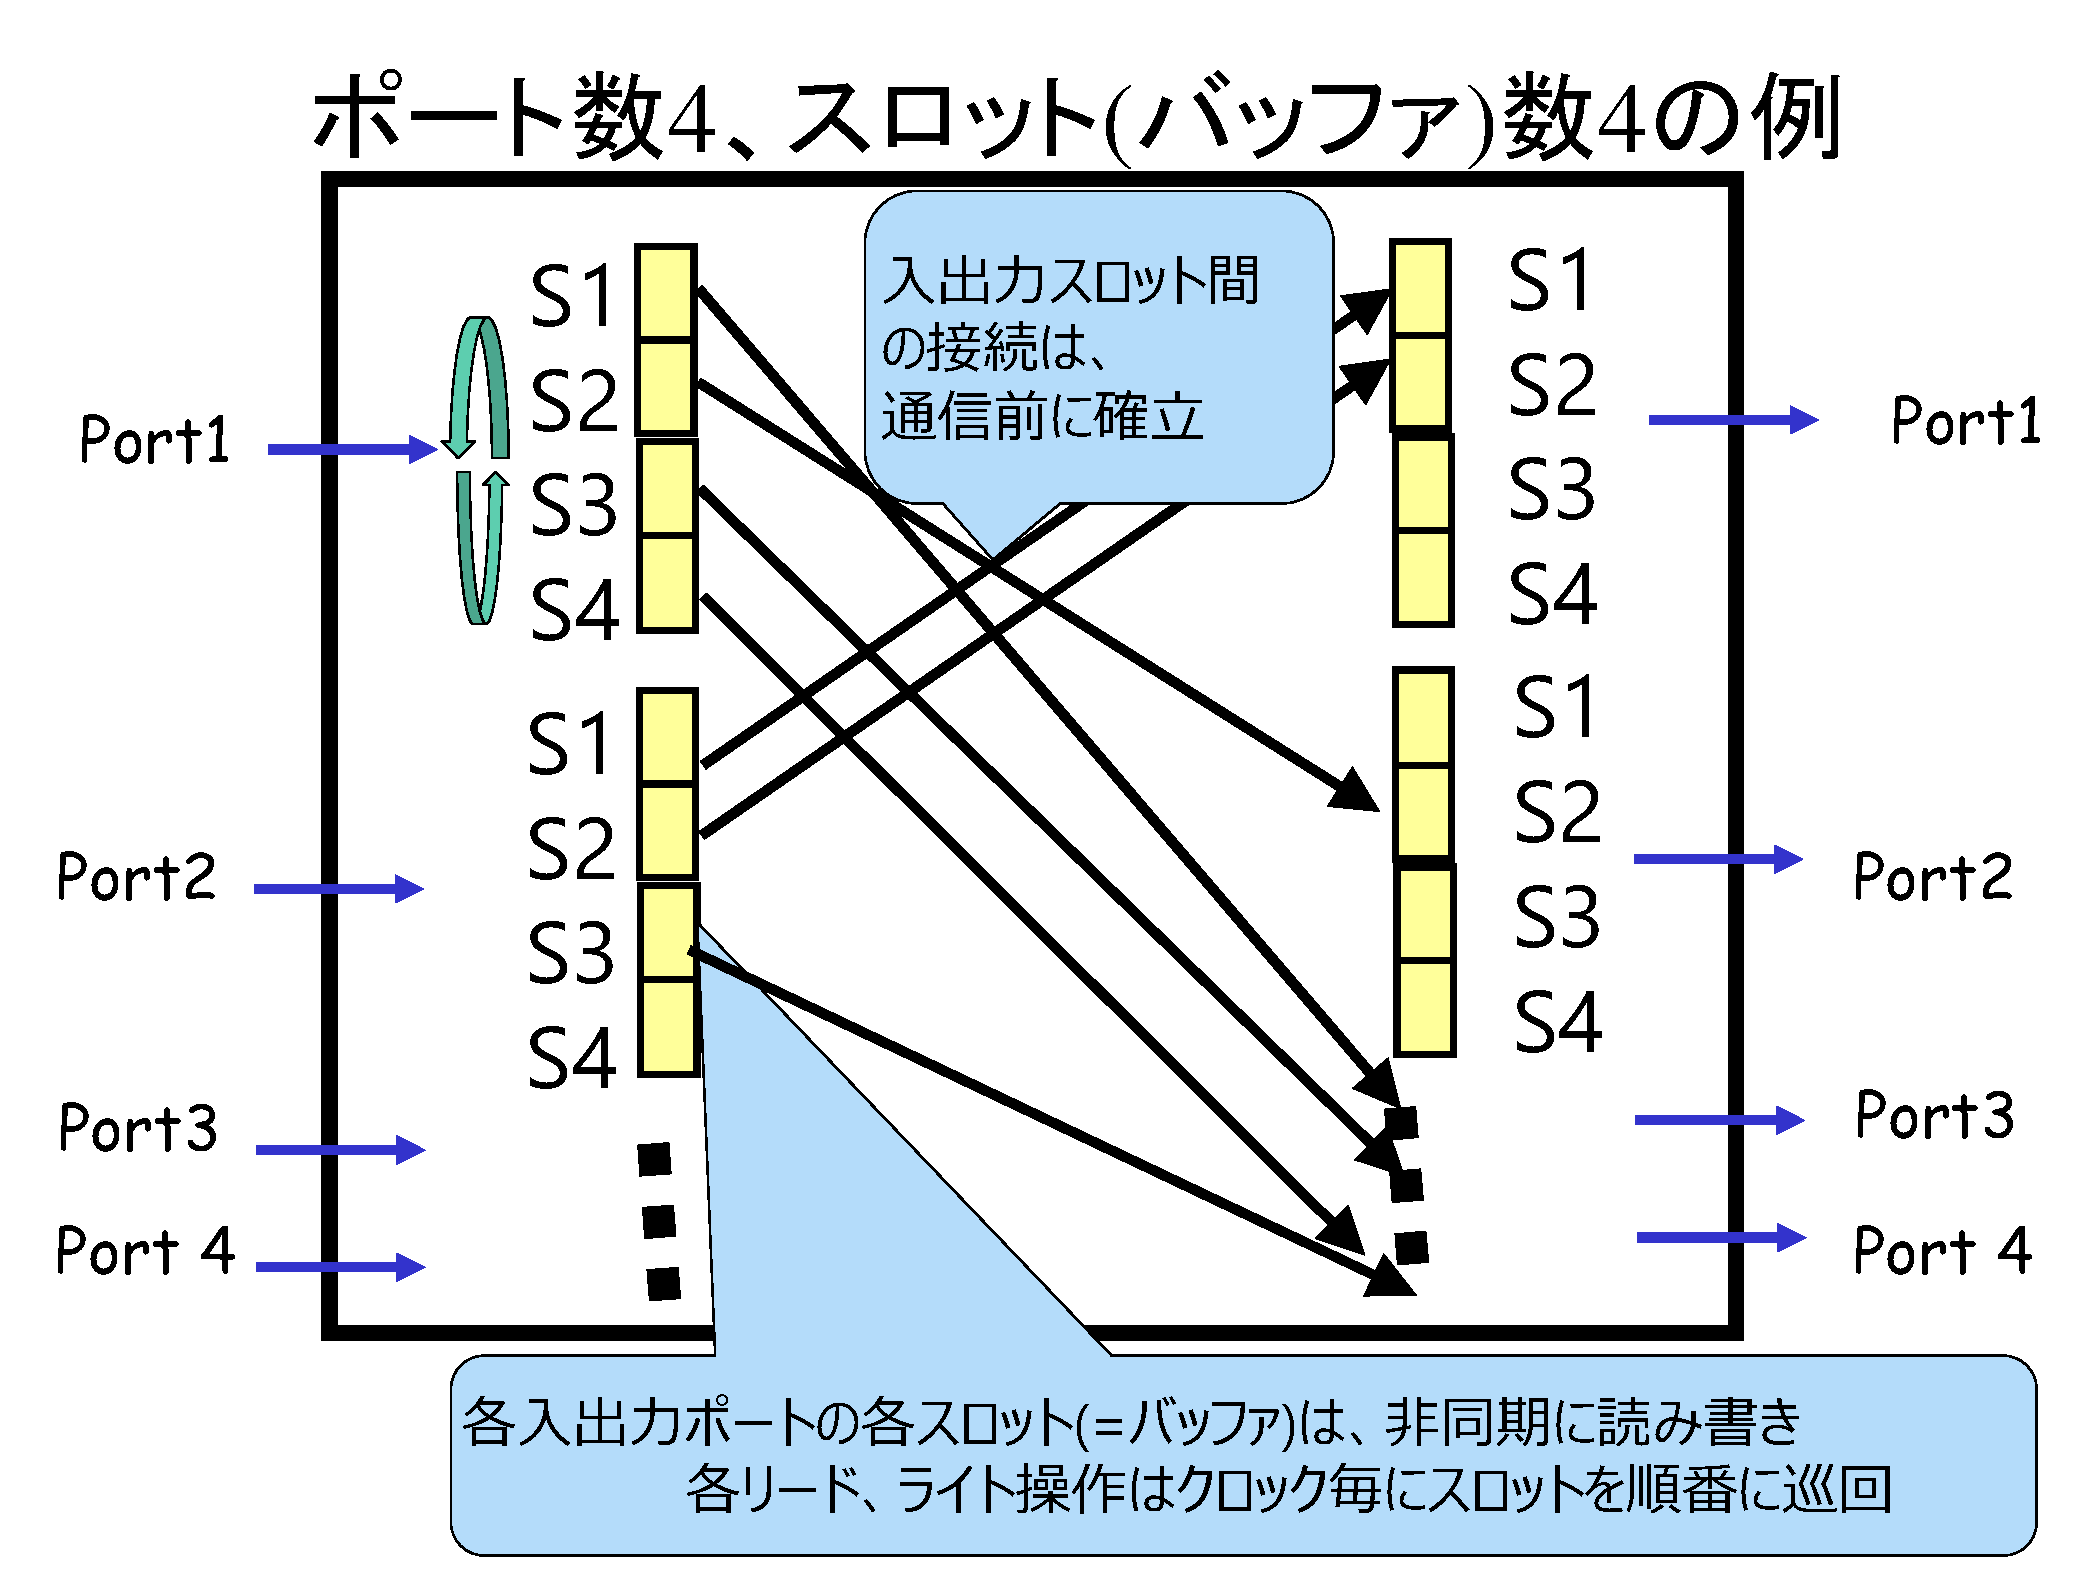
\includegraphics[width=1.0\columnwidth]{fig/switch.eps}
  \caption{FiC-SW1のサーキットスイッチ}
%  \ecaption{Static analysis result of an example pattern}
  \label{fig_switch}  
 \end{center}  
\end{figure}

\begin{figure}[ht]  
 \begin{center}   
	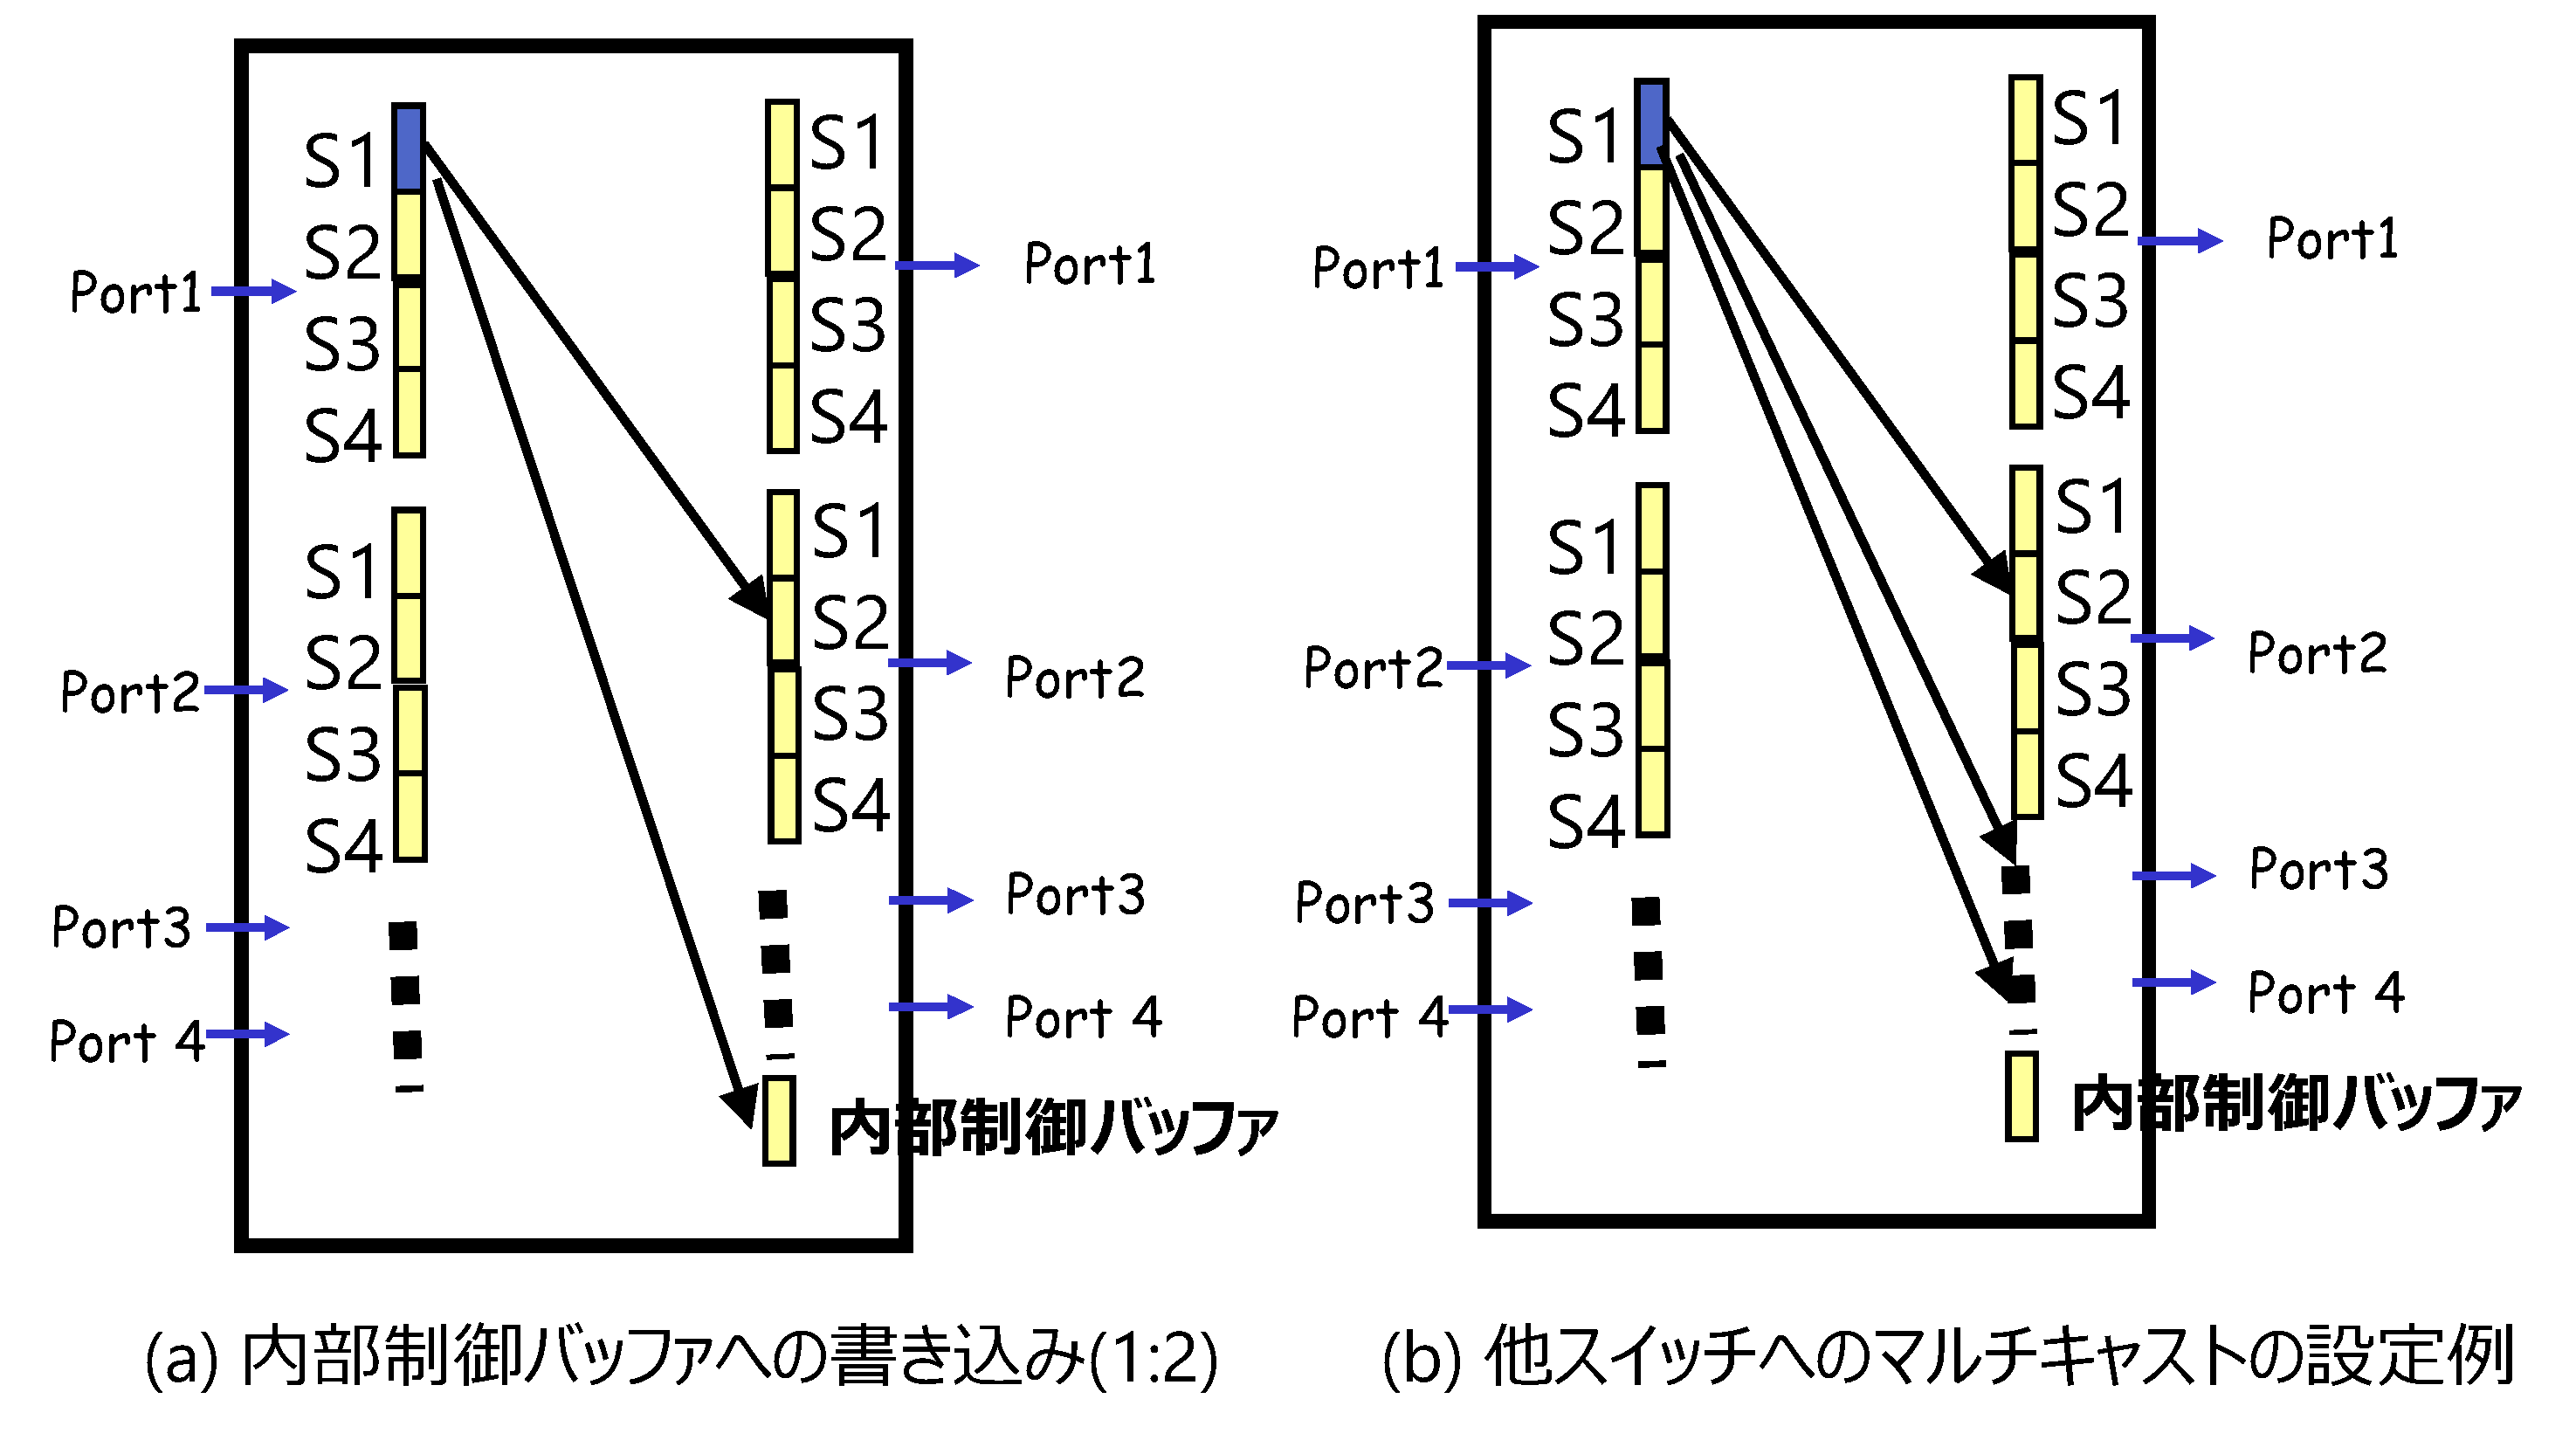
\includegraphics[width=1.0\columnwidth]{fig/multicast.eps}
  \caption{入出力スロットの再接続の例}
%  \ecaption{Static analysis result of an example pattern}
  \label{fig_multicast}  
 \end{center}  
\end{figure}

